\begin{figure}[h]
 \centering
 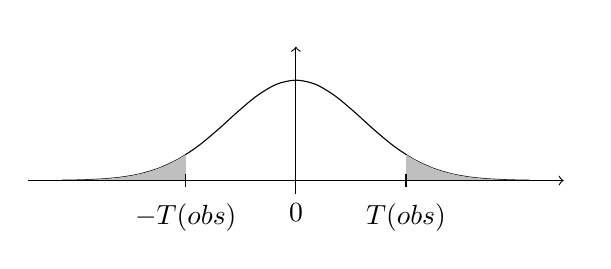
\begin{tikzpicture}[scale=0.85]
    % Draw the normal distribution curve
    \draw[domain=-3.5:3.5, smooth, variable=\x] plot ({\x}, {1.5*exp(-0.5*\x*\x)});

    % Shade the right tail area
    \fill[gray!50] (1.645,0) -- plot[domain=1.645:3.5, smooth, variable=\x] ({\x}, {1.5*exp(-0.5*\x*\x)}) -- (3.5,0) -- cycle;

    % Shade the left tail area
    \fill[gray!50] (-1.645,0) -- plot[domain=-1.645:-3.5, smooth, variable=\x] ({\x}, {1.5*exp(-0.5*\x*\x)}) -- (-3.5,0) -- cycle;

    % Label for the mean
    \node[below] at (0,-0.2) {$0$};

    % Label for the right critical value
    \node[below] at (1.645,-0.2) {$T(\text{obs})$};

    % Label for the left critical value
    \node[below] at (-1.645, -0.2) {$-T(\text{obs})$};

    % Axes
    \draw[->] (-4,0) -- (4,0) node[right] {};
    \draw[->] (0,-0.2) -- (0,2) node[above] {};

    \draw[-] (1.645,-0.1) -- (1.645,0.1) node[right] {};
    \draw[-] (-1.645,-0.1) -- (-1.645,0.1) node[right] {};


\end{tikzpicture}
\caption{
Density of standard normal $Z\sim \calN(0,1)$ random variable. Shaded area is equal to $p$-value $\Prob(|Z|\geq T(\text{obs}))$.
}\label{fig:normal_distr_two_sided}
\end{figure}



